\documentclass[tikz,border=2pt]{standalone}
\usepackage{tikz}

\begin{document}
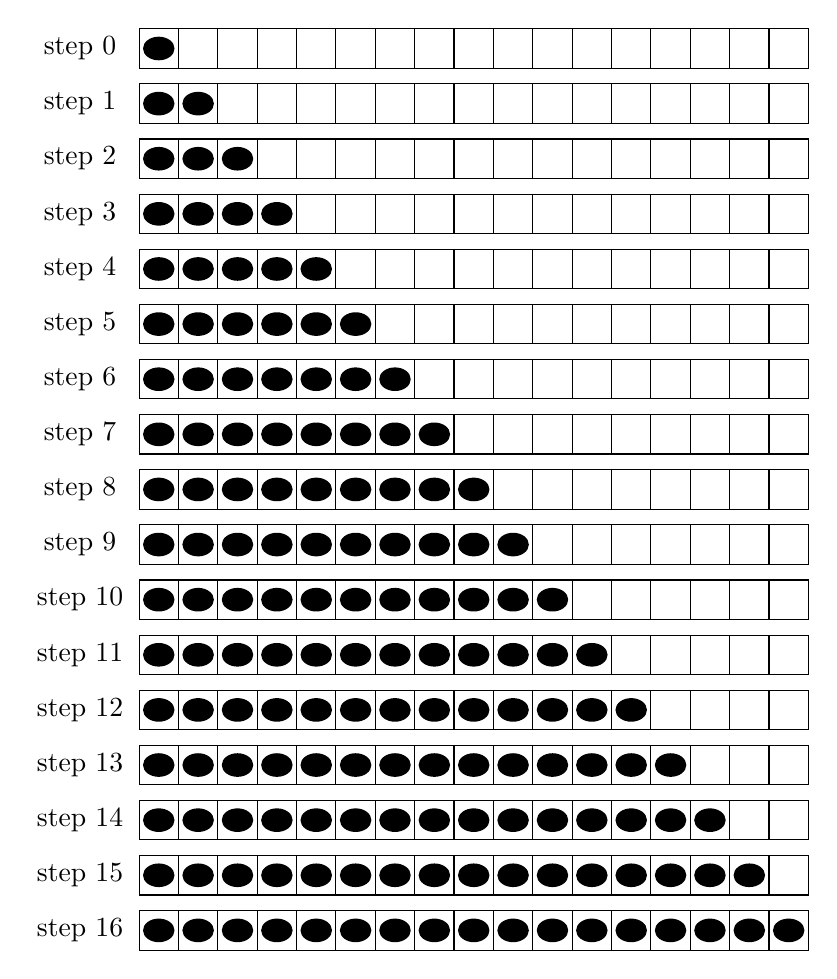
\begin{tikzpicture}[scale=1.0]

\foreach[evaluate={\j=int(16-\y)}] \y in {0,...,16}{
	\node at (-1, 0.7*\y) {step \j};
	\foreach \x in {0,...,16}{
		\draw (0.5*\x-0.25, 0.7*\y-0.25) rectangle (0.5*\x+0.25, 0.7*\y+0.25);
	}
	\foreach \x in {0,...,\j}{
		\fill (0.5*\x, 0.7*\y)  ellipse (0.2 and 0.15);
	}
}

\end{tikzpicture}
\end{document}
